% Template for ICIP-2009 paper; to be used with:
%          spconf.sty  - ICASSP/ICIP LaTeX style file, and
%          IEEEbib.bst - IEEE bibliography style file.
% --------------------------------------------------------------------------
\documentclass{article}
\usepackage{spconf,amsmath,epsfig}

% Example definitions.
% --------------------
\def\x{{\mathbf x}}
\def\L{{\cal L}}

% Title.
% ------
\title{PEDESTRIAN DETECTION USING HAAR-LIKE FEATURES}
%
% Single address.
% ---------------
\name{Tim Besard, Ruben Schollaert, Dimitri Roose, Sebastiaan Labijn}
%\thanks{Thanks to University College Ghent for funding.}
\address{University College Ghent\\Applied Engineering\\Campus Schoonmeersen, Valentin Vaerwyckweg 1, 9000 Gent}


\begin{document}
%\ninept
%
\maketitle
%
\begin{abstract}
%The abstract should appear at the top of the left-hand column of text, about
%0.5 inch (12 mm) below the title area and no more than 3.125 inches (80 mm) in
%length.  Leave a 0.5 inch (12 mm) space between the end of the abstract and the
%beginning of the main text.  The abstract should contain about 100 to 150
%words, and should be identical to the abstract text submitted electronically
%along with the paper cover sheet.  All manuscripts must be in English, printed
%in black ink.
% Begin abstract
In this paper a solution for pedestrian detection is described using Haar-like features. It is being developed to be used in a tram collision advoidance project. 
\end{abstract}
%
\begin{keywords}
Pedestrian Detection, Haar-like Features, AdaBoost Classification
\end{keywords}
%
\section{Introduction}
\label{sec:intro}
Object detection is a very important element in computer vision areas. The goal is to find a predefined object in a set of images or video frames. This task can be fulfilled using template matching techniques extracting certain image features such as edges, color regions, textures and contours.
\par
Alas for complex objects such as pedestrians these features are hard to find due the great variety of instances of these pedestrians. The major problems causing this huge variety lie in~\cite{monteiro2006vision}:
\begin{itemize}
\item The size, color and style of pedestrian clothing are very diverse.
\item Pedestrians are nong-rigid bodies. Their shape and size differ greatly and therefore they are more complex that rigid objects.
\item Not only the pedestrians themselves are part of the problem. The background can cause cluttering and due this parts of it could be mistaken for pedestrians.
\item Illumination and weather conditions can lower the distinction between background and pedestrian.
\item Also the lack in motion due the slow speed of pedestrians hardens the possibility for them to be detected.
\end{itemize}
Instead of using the template matching approach, another possible encounter has been stated by Viola and Jones~\cite{viola2001rapid}.
\section{How it works}
This approach uses statistical models, so called classifiers. These are created by extensive training using a pool of test images. These pools consists of "positive" and "negative" samples, respectively images that contain pedestrians and images that don't. From these sample images features are extracted and the features which classify the pedestrians are selected. These are the so called Haar-like features. The general flow of this process is shown in Figure~\ref{fig:flowchart}.
\begin{figure}[h!]
\centering
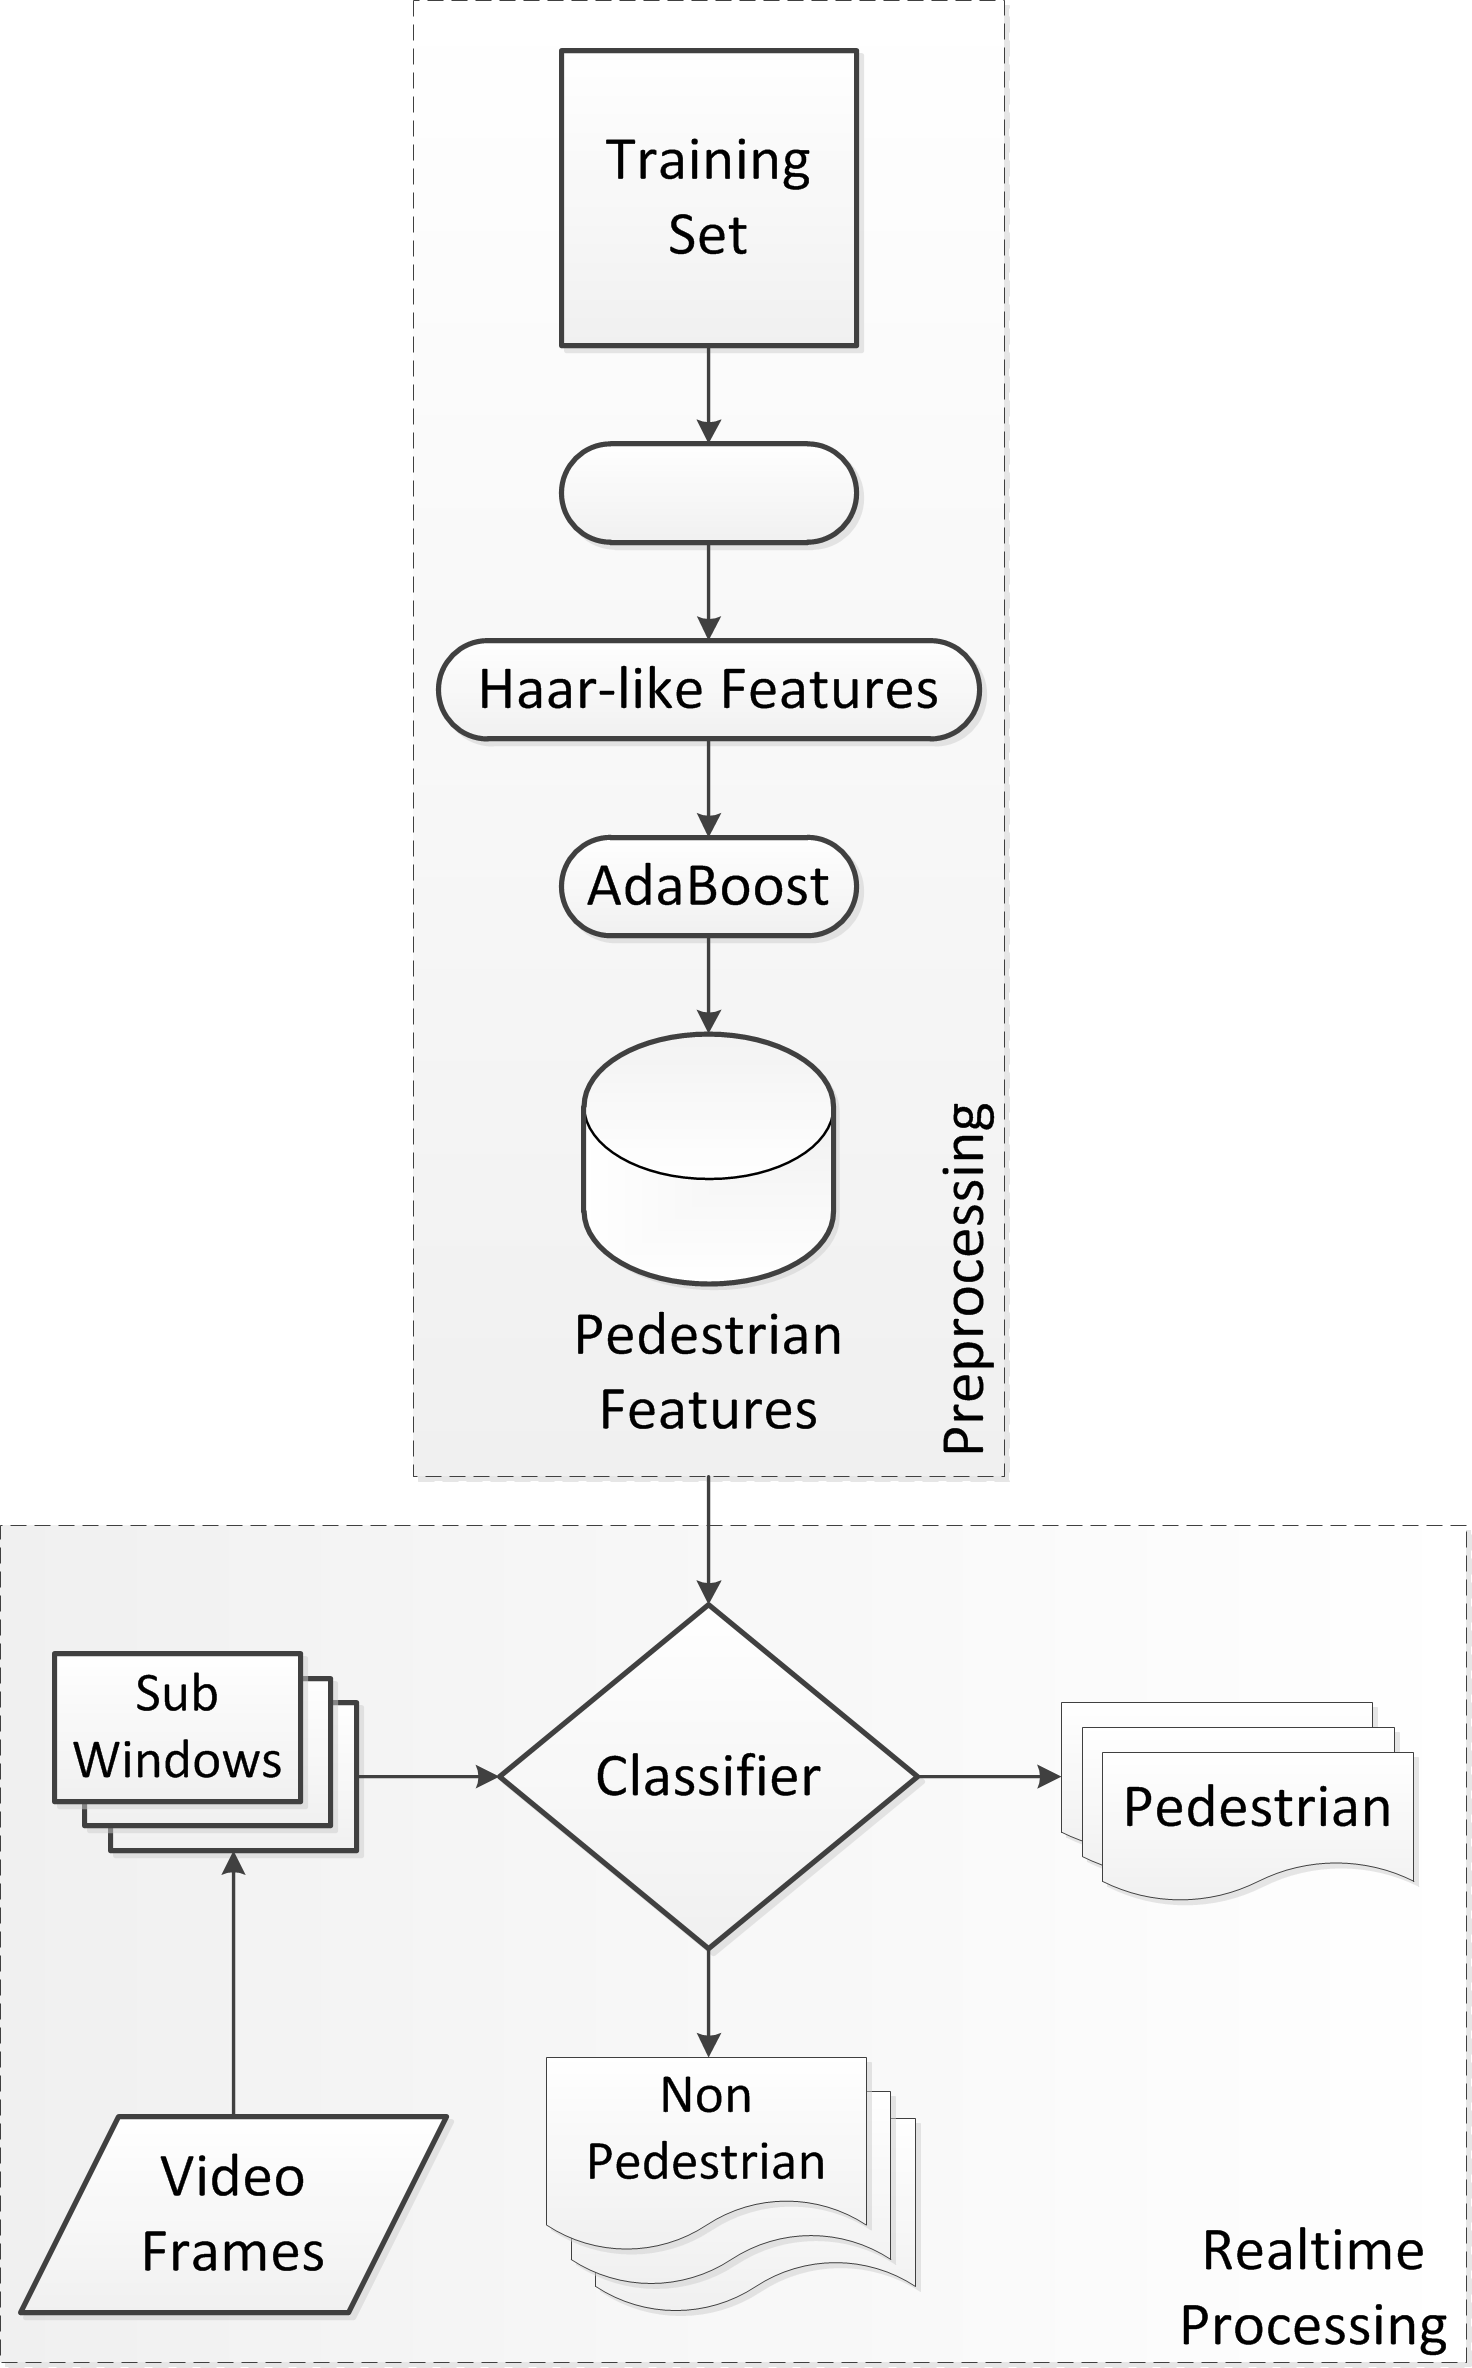
\includegraphics[scale=0.5]{HaarTrainingFlowChart.png}
\caption{Flowchart for detecting pedestrians.}
\label{fig:flowchart}
\end{figure}

%The Haar-like features (so called because they are computed
%similarly to the coefficients of Haar wavelet trans-
%forms) and a large set of very simple “weak”
%classifiers, that use a single feature to classify
%the image as pedestrian or non-pedestrian, were
%used to extract the features characteristics of the
%pedestrians.
%
%and extended by Lienhart et al. [1,2]. In one image
%sub-window, the total number of Haar-like fea-
%tures is very large, far larger than the number of
%pixels. In order to ensure a fast classification, the
%learning process must exclude a large majority of
%the available features, and focus on a small set of
%critical features. A variant of AdaBoost [4] is used
%for making those features selection (see Figure 1).
%Training Set
%Normalization
%A similar methodology combining Haar-like fea-
%tures and the AdaBoost algorithm, proposed by
%Viola et. al. to detect faces, is proposed here to
%detect pedestrians on the road.

% TODO Per sectie beetje uitleg geven.
\section{Haar-like features}
A feature is represented by a shape composed of two or three black and white rectangles joined together. These rectangles can be turned horizontal, vertical or diagonal.
%Each feature is represented by a template (shape
%of the feature), its coordinate relative to the search
%window origin and the size of the feature (its
%scale). A subset of the features prototypes used
%is shown in Figure 2.
%Each feature is composed of two or three “black”
%and “white” rectangles joined together - these
%rectangles can be up-right or rotated by 45 de-
%grees. The Haar-like features value is calculated
%as a weighted sum of two components: the pixel
%gray level values sum over the black rectangle and
%the sum over the whole feature area (all black and
%white areas). The weights of these two compo-
%nents are of opposite signs and for normalization
%purpose, their absolute values are inversely pro-
%portional to the areas.
%Fig. 2. Subset of the Haar-like features prototypes
%used in the pedestrian detection.
%2.1 Integral Image
%Hundreds of features are used in a real and ro-
%bust classifier. Therefore,the direct computation
%of pixel sums over multiple rectangles would make
%the detection task very slow and not suitable
%for real-time applications. Viola et al. [3] intro-
%duced an efficient method for computing the sums
%quickly. The integral image, Summed Area Table
%(SAT ), is computed over the whole image I, and
%the SAT is defined by the Equation 1.
%h
%1
%SAT (x, y) =
%I(i, j)
%(1)
%i<x,j<y
%The pixel sum over a generic rectangle
%r = {(x, y) , x0 ≤ x < x0 + w, y0 ≤ y < y0 + h}
%can then be computed using the SAT. The sum is
%done by using the rectangle corners coordinates,
%as described in the Equation 2.
%S(r) = SAT (x0 + w, y0 + h) − SAT (x0 + w, y0 )
%− SAT (x0 , y0 + h) + SAT (x0 , y0 ) (2)
%For rotated features/rectangles, a separate “ro-
%tated” integral image must be computed, as Lien-
%hart et al. [2] describes.
\label{sec:format}

%TODO: Schema met hier van de flow:\\
Building the boosted classifiers takes the most time because it requires a lot of training data and iterations in the AdaBoost algorithm. Once these classifiers are built, the detection is capable of processing images extremely rapidly and achieving high detection rates~\cite{viola2001rapid}.

\section{Training a cascade of classifiers}

\section{Adaboost Algorithm}


\section{OpenCV Haartraining}
To create and test the cascade of boosted classifiers based on haar-like features we are using OpenCV \cite{opencv_library}. OpenCV provides us programs that we can use to create our own classifiers.

\subsection{Create samples}
Before we can start creating samples we need positive images, these are images which contain pedestrians without much variations in the illumination, if there are too many variations the resulting detector will not work well.
Besides the positive images we also need negative images and testing images. The testing images are images in combination with the location of the pedestrians. We used the CBCL PEDESTRIAN DATABASE \#1 from MIT which contains 924 images.
From one image we can create several samples by using distortion, we can use the createsamples program delivered by OpenCV for this. For example 

createsamples -img image.png -num 10 -bg negatives.dat -vec samples.vec -w 64 -h 128

will generate 10 samples out of one image.
The file 'negatives.dat' is a file containing a list of the negative images used.

For the test images we need to create a file which includes the location of the pedestrian in each image. This file will just hold the x and y coordinates in combination with the height and width of the pedestrian.
After these steps we can start creating the testing samples, these are created as follows:

createsamples -img image.png -num 10 -bg negatives.dat -info test.dat -maxxangle 0.6 -maxyangle 0 -maxzangle 0.3 -maxidev 100 -bgcolor 0 -bgthresh 0

The output will be cropped pedestrians placed on top of negative samples, a description file with the coordinates of the cropped pedestrian in the new image will also be available.




\subsection{Train}
To train our classifier we can use the haartraining utility. The following training takes about four days.

haartraining -data haarcascade -vec samples.vec -bg negatives.dat -nstages 20 -nsplits 2 -npos 5000 -nneg 2500 -w 20 -h 80 -nonsym -mem 512 -mode ALL

We use the '-nonsym' parameter because people don't have a symmetric body structure in all poses. If we would be making classifiers for a symmetric object we would use the default, so only half of the image will be processed  thus speeding up the training. We also specified the '-mode ALL', this means the haartraining will look for all haar-like features, default will only look for upright features.
Increasing the number of stages (-nstages 20) will not necessarily produce a better result. If the default threshold of minimum 99.5\% hitrate or the maximum false alarm of 50\% is reached, the training will stop.
When the training is finished, OpenCV will generate an XML outputfile.
\subsection{Test}
OpenCV also has a program to test the performance of the generated classifiers. This program is called 'performance'. Testing the XML can be done like this:
performance -data haarcascade.xml -info tests.dat -ni
The tests.dat file contains a list of testing images and the 'ni' parameter is used so the performance-utility will not output any detection images.
The performance utility will then output the number of correct detections, the number of missed or false negatives and the number of false positives.
\section{Experimental results}

\section{Conclusion}


\section{ILLUSTRATIONS, GRAPHS, AND PHOTOGRAPHS}
\label{sec:illust}

Illustrations must appear within the designated margins.  They may span the two
columns.  If possible, position illustrations at the top of columns, rather
than in the middle or at the bottom.  Caption and number every illustration.
All halftone illustrations must be clear black and white prints.  Colors may be
used, but they should be selected so as to be readable when printed on a
black-only printer.

Since there are many ways, often incompatible, of including images (e.g., with
experimental results) in a LaTeX document, below is an example of how to do
this \cite{Lamp86}.

% Below is an example of how to insert images. Delete the ``\vspace'' line,
% uncomment the preceding line ``\centerline...'' and replace ``imageX.ps''
% with a suitable PostScript file name.
% -------------------------------------------------------------------------
\begin{figure}[htb]

\begin{minipage}[b]{1.0\linewidth}
  \centering
% \centerline{\epsfig{figure=image1.ps,width=8.5cm}}
  \vspace{2.0cm}
  \centerline{(a) Result 1}\medskip
\end{minipage}
%
\begin{minipage}[b]{.48\linewidth}
  \centering
% \centerline{\epsfig{figure=image3.ps,width=4.0cm}}
  \vspace{1.5cm}
  \centerline{(b) Results 3}\medskip
\end{minipage}
\hfill
\begin{minipage}[b]{0.48\linewidth}
  \centering
% \centerline{\epsfig{figure=image4.ps,width=4.0cm}}
  \vspace{1.5cm}
  \centerline{(c) Result 4}\medskip
\end{minipage}
%
\caption{Example of placing a figure with experimental results.}
\label{fig:res}
%
\end{figure}

% To start a new column (but not a new page) and help balance the last-page
% column length use \vfill\pagebreak.
% -------------------------------------------------------------------------
\vfill
\pagebreak


\section{FOOTNOTES}
\label{sec:foot}

Use footnotes sparingly (or not at all!) and place them at the bottom of the
column on the page on which they are referenced. Use Times 9-point type,
single-spaced. To help your readers, avoid using footnotes altogether and
include necessary peripheral observations in the text (within parentheses, if
you prefer, as in this sentence).


\section{COPYRIGHT FORMS}
\label{sec:copyright}

You must include your fully completed, signed IEEE copyright release form when
you submit your paper. We {\bf must} have this form before your paper can be
published in the proceedings.  The copyright form is available as a Word file,
a PDF file, and an HTML file. You can also use the form sent with your author
kit.

\bibliographystyle{IEEEbib}
\bibliography{bibliografie}

\end{document}
